\begin{block}{}
    \vspace{-3cm}
    \begin{figure}\centering
        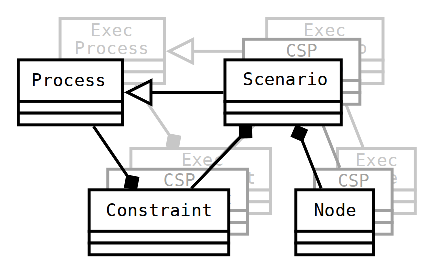
\includegraphics[width=0.7\columnwidth]{images/orga3.eps}
        \caption{Organisation des graphes d'entités - composants}
        \label{fig.uml}
    \end{figure}
\end{block}
\begin{block}{Prochaines étapes}
    \small
    \begin{itemize}
        %\item Scripting intégré : intégration d'un langage de haut-niveau interprété (\textbf{QML}) pour prototyper plus simplement sur le logiciel.
        \item Implémentation audio plus poussée via \textbf{libaudiostream}\cite{letz_specification_2014} qui crée un graphe semblable à celui d'i-score.
        \item Travail en cours sur modèles et \textbf{processus spatiaux} : écriture avec des données multi-dimensionnelles.
    \end{itemize}
\end{block}